% Extension slides for final_project_beamer_100_pages.tex (milestone M8), added 2026-11-27.
% Input with % Extension slides for final_project_beamer_100_pages.tex (milestone M8), added 2026-11-27.
% Input with % Extension slides for final_project_beamer_100_pages.tex (milestone M8), added 2026-11-27.
% Input with % Extension slides for final_project_beamer_100_pages.tex (milestone M8), added 2026-11-27.
% Input with \input{docs/report_drafts/beamer_extension_20261127} after the pilot's Results section.
% Numbers come from the report chapter docs/report_drafts/results_title_alignment_20261106.tex and the
% dated reports it cites (docs/walk_forward_reward_20261106.md, docs/pit_walk_forward_20261107.md,
% docs/bistka_300k_results_20261125.md, docs/final_test_results_20261125.md,
% docs/holdout_results_20261126.md, docs/source_ablation_20261127.md, docs/architecture_ablation_20261127.md).

\section{Extension: Long-Term, Point-in-Time Results}

\begin{frame}{What Changed After The Pilot}
\begin{itemize}
  \item \textbf{Objective:} a long-term reward (log return, a differential Sharpe term, minus new drawdown) with weekly decisions, instead of the one-day reward.
  \item \textbf{Accounting:} self-financing, 0.20\% cost per side, costs charged once.
  \item \textbf{Data:} 2012--2024 history; the official point-in-time SET50 membership (34 lists, 227 tickers).
  \item \textbf{Evaluation:} seven one-year walk-forward folds (2016--2022), each trained only on earlier years; then the 2023--2024 test years and a sealed holdout (2025 to 4 November 2026), each read once.
  \item \textbf{Compute:} the large runs on BistKA (210, 35 and 147 models in three jobs).
\end{itemize}
\end{frame}

\begin{frame}{Reward And Rebalancing Designs (2020--2022)}
\begin{center}
\scriptsize
\begin{tabular}{lrr}
\toprule
Design (PPO, 3 seeds, five stocks) & Return 2020--2022 & Costs \\
\midrule
V2 objective (one-day reward) & $-48.8\% \pm 7.6$ & 75.3\% \\
Daily simple return, fixed accounting & $-41.9\% \pm 6.9$ & 56.0\% \\
Log return, weekly & $-2.8\% \pm 5.8$ & 16.0\% \\
Plan reward, weekly & $-8.8\% \pm 17.2$ & 11.7\% \\
Plan reward, weekly, per-stock LSTM & $+1.9\% \pm 1.1$ & 1.6\% \\
\midrule
SET50 ETF buy-and-hold & $+9.0\%$ & 0.2\% \\
Equal weight, monthly & $+2.7\%$ & 0.5\% \\
\bottomrule
\end{tabular}
\end{center}
\begin{itemize}
  \item The pilot lost money mainly by overtrading. Weekly long-horizon rewards cut costs by 79--94\%.
\end{itemize}
\end{frame}

\begin{frame}{Seven-Year Walk-Forward, Five Stocks}
\begin{center}
\scriptsize
\begin{tabular}{lrrr}
\toprule
Strategy (2016--2022, 7 folds) & Annual return & Years ahead of ETF & Max DD \\
\midrule
LSTM forecast, top two & 13.8\% & 5/7 & $-17.0\%$ \\
Ridge forecast, top two & 12.8\% & 5/7 & $-16.8\%$ \\
Equal weight, monthly & 10.1\% & 4/7 & $-13.9\%$ \\
DRL, plan reward + LSTM (5 seeds) & 7.6\% & 3/7 & $-11.1\%$ \\
SET50 ETF buy-and-hold & 7.1\% & -- & $-11.3\%$ \\
\bottomrule
\end{tabular}
\end{center}
\begin{itemize}
  \item DRL had the lowest drawdown but did not beat equal weight or the forecasters.
  \item No difference is statistically significant (block bootstrap on daily returns).
\end{itemize}
\end{frame}

\begin{frame}{Why The Universe Matters}
\begin{itemize}
  \item Five stocks, or today's SET50 names, are chosen with hindsight.
  \item Equal weight over the \textbf{2024 SET50 names}: 12.2\% a year, ahead of the ETF in 7 of 7 years.
  \item Equal weight over \textbf{each session's actual members}: 5.6\% a year, ahead in 2 of 7.
  \item Hindsight therefore added 6.6 points a year. Every later result uses the actual members.
  \item Gap: 38 of the 227 tickers, mostly delisted or merged, have no Yahoo prices (13\% of member-sessions).
\end{itemize}
\end{frame}

\begin{frame}{Point-in-Time SET50: Design Steps}
\begin{center}
\scriptsize
\begin{tabular}{lrr}
\toprule
Design (validation 2016--2022) & Annual return & Max DD \\
\midrule
DRL, slots ordered by traded value & $-1.1\%$ & $-14.8\%$ \\
+ sticky slot order & 3.7\% & $-14.2\%$ \\
+ shared-weight actor (scores every stock alike) & 4.6\% & $-11.7\%$ \\
+ seed ensemble and 0.5-point no-trade band & 5.5\% & $-11.3\%$ \\
\textbf{+ cash capped at 20\% (locked design)} & \textbf{5.0\%} & $-12.0\%$ \\
Shared actor at 300k timesteps, ensemble + band & 3.9\% & $-7.0\%$ \\
\midrule
Equal weight (point-in-time), monthly & 5.6\% & $-12.7\%$ \\
SET50 ETF buy-and-hold & 7.1\% & $-11.2\%$ \\
Momentum / inverse volatility / minimum variance & 5.3 / 5.0 / 4.0\% & \\
\bottomrule
\end{tabular}
\end{center}
\begin{itemize}
  \item No design beat equal weight; none of these differences is significant except the first two (worse).
\end{itemize}
\end{frame}

\begin{frame}{Point-in-Time SET50: Chained Value}
\begin{center}
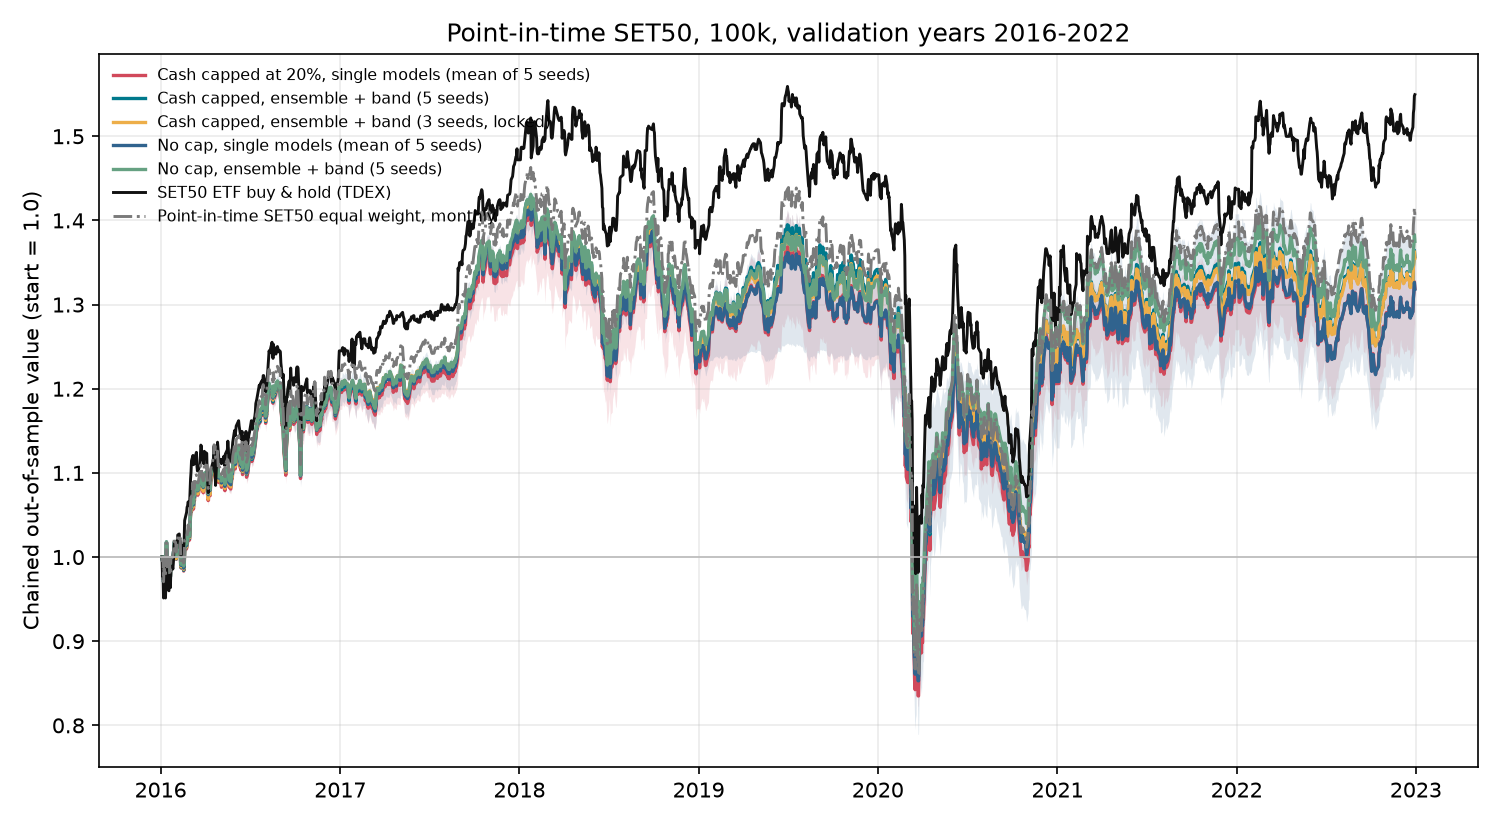
\includegraphics[width=\textwidth]{docs/figures/pit_cash_cap_100k_5seeds_chained_equity_20261126.png}
\end{center}
\footnotesize The cash-capped design (five seeds: single models and the seed ensemble with the band) and the uncapped design, against equal weight and the ETF; each year uses models trained only on earlier years, net of costs.
\end{frame}

\begin{frame}{What The Agent Learned}
\begin{itemize}
  \item \textbf{Close to equal weight:} daily correlation 0.998, about 44 effective holdings of 44.5 tradable members, no weight above about 3\%.
  \item \textbf{Less trading:} the seed ensemble with the band turned over 0.6 times its capital a year after entry (equal weight 0.9).
  \item \textbf{Cash was a learned bias:} 15 models across four designs held 36--94\% cash; shuffling their inputs moved that cash by 5 points or less in 12 of them.
  \item \textbf{The 20\% cash cap} removed the cash-heavy models but not the gap to equal weight, which lies in costs and stock tilts that do not pay.
\end{itemize}
\end{frame}

\begin{frame}{Five Algorithms On BistKA (300k Timesteps, 5 Seeds)}
\begin{center}
\scriptsize
\begin{tabular}{lrrrrr}
\toprule
Five stocks, 2016--2022 & A2C & PPO & SAC & TD3 & DDPG \\
\midrule
Annual return & \textbf{8.7\%} & 4.4\% & 0.3\% & $-0.9\%$ & $-1.4\%$ \\
Costs a year (points) & 0.9 & 1.3 & 6.1 & 6.6 & 6.3 \\
Turnover a year & 4.3 & 6.0 & 29.4 & 32.1 & 30.5 \\
Hours per model & 0.4 & 1.1 & 17.2 & 10.7 & 13.9 \\
\bottomrule
\end{tabular}
\end{center}
\begin{itemize}
  \item ETF 7.1\%, equal weight 10.1\%.
  \item Off-policy algorithms overtraded; TD3 and DDPG are significantly worse than the ETF, equal weight and PPO.
  \item A2C is best and cheapest, but not significantly better than PPO or either benchmark.
\end{itemize}
\end{frame}

\begin{frame}{Longer Training Did Not Help}
\begin{itemize}
  \item \textbf{PPO, five stocks:} 7.6\% a year at 100k timesteps, 4.4\% at 300k; average cash rose from 20\% to 39\%. The only significant budget effect ($-0.16$ Sharpe).
  \item \textbf{Point-in-time, no cap:} at 300k, 17 of 35 models held 45--98\% cash; the ensemble made 3.9\% a year with a smaller drawdown.
  \item \textbf{Point-in-time, 20\% cap:} cash held to 8.7\%, but the ensemble made 4.9\% against 5.0\% at 100k (Sharpe 0.35 against 0.36).
  \item 100k timesteps is enough for the locked design.
\end{itemize}
\end{frame}

\begin{frame}{Choosing The Design Before Looking}
\begin{itemize}
  \item \textbf{Rule fixed in advance (decision 7):} median over years of the annual excess log return over equal weight; if no design scores above zero, equal weight is selected.
  \item \textbf{Outcome:} no DRL design scored above zero in either universe, so the rule selects equal weight.
  \item \textbf{Evaluated anyway:} the best DRL designs, the cash-capped point-in-time ensemble with the band and five-stock A2C at 300k.
  \item \textbf{Locks and gates:} each evaluation ran once from an approved lock file; every opening is in \texttt{results/FINAL\_TEST\_LEDGER.jsonl}.
\end{itemize}
\end{frame}

\begin{frame}{Test Years 2023--2024 (Run Once)}
\begin{center}
\scriptsize
\begin{tabular}{lrrrr}
\toprule
Strategy & 2023 & 2024 & Two years & Sharpe \\
\midrule
\multicolumn{5}{l}{\emph{Point-in-time SET50}} \\
DRL, cash-capped, ensemble + band & $-11.4\%$ & $-6.7\%$ & 0.827 & $-0.80$ \\
Equal weight, monthly & $-13.5\%$ & $-7.6\%$ & 0.799 & $-0.86$ \\
\multicolumn{5}{l}{\emph{Five starter stocks}} \\
DRL, A2C, 300k & $-1.9\%$ & $+4.4\%$ & 1.026 & 0.19 \\
Equal weight, monthly & $-3.6\%$ & $+10.1\%$ & 1.061 & 0.33 \\
\midrule
SET50 ETF buy-and-hold & $-9.1\%$ & $+8.2\%$ & 0.984 & $-0.01$ \\
\bottomrule
\end{tabular}
\end{center}
\begin{itemize}
  \item Point-in-time DRL was ahead of equal weight in both years, not significantly, and behind the ETF.
  \item Yahoo's 2024 prices have stale rows on real trading days; disclosed, results stand as locked.
\end{itemize}
\end{frame}

\begin{frame}{Sealed Holdout, 2025 To 4 November 2026 (Run Once)}
\begin{center}
\scriptsize
\begin{tabular}{lrrrr}
\toprule
Strategy & 2025 & 2026 to 4 Nov & Chained & Sharpe \\
\midrule
\multicolumn{5}{l}{\emph{Point-in-time SET50 (2024 H2 list held fixed)}} \\
DRL, cash-capped, ensemble + band & $-8.8\%$ & $+23.7\%$ & 1.128 & 0.48 \\
Equal weight, monthly & $-8.8\%$ & $+29.7\%$ & 1.183 & 0.60 \\
\multicolumn{5}{l}{\emph{Five starter stocks}} \\
DRL, A2C, 300k & $+0.7\%$ & $+14.3\%$ & 1.153 & 0.59 \\
Equal weight, monthly & $+6.0\%$ & $+20.8\%$ & 1.281 & 0.94 \\
\midrule
SET50 ETF buy-and-hold & $-2.8\%$ & $+24.9\%$ & 1.214 & 0.75 \\
\bottomrule
\end{tabular}
\end{center}
\begin{itemize}
  \item The locked design matched equal weight in the falling year and trailed it in the rally, holding cash up to its cap.
  \item Its Sharpe shortfall against equal weight is \textbf{significant}: $-0.12$ ($-0.23$ to $-0.01$).
\end{itemize}
\end{frame}

\begin{frame}{Sealed Holdout: Chained Value}
\begin{center}
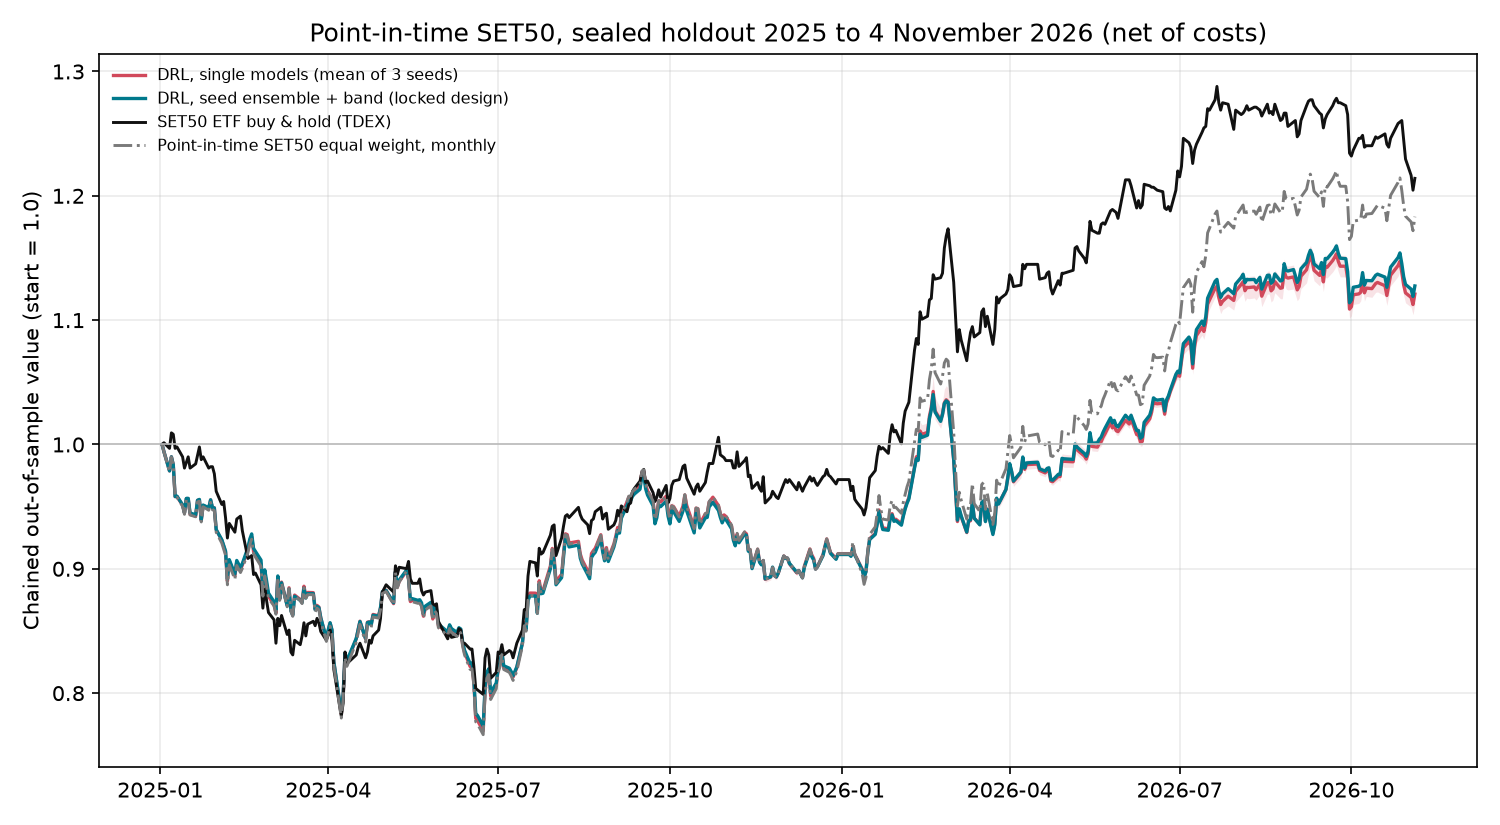
\includegraphics[width=\textwidth]{docs/figures/holdout_pit_chained_equity_20261126.png}
\end{center}
\footnotesize Locked point-in-time design (seed ensemble with the band, and its single models) against equal weight and the ETF; models trained only on earlier years, net of costs.
\end{frame}

\begin{frame}{Checks After The Holdout (Validation Years Only)}
\begin{center}
\scriptsize
\begin{tabular}{lrrr}
\toprule
Locked design with one change (5 seeds) & Single & Ensemble & Sharpe diff. (single) \\
\midrule
Locked: LSTM, technical + ETF inputs & 4.6\% & 5.0\% & -- \\
MLP encoder instead of LSTM & 4.4\% & 5.1\% & $-0.006$ \\
Technical inputs only & 4.5\% & 5.2\% & $-0.001$ \\
+ BOT policy rate & 4.6\% & 5.2\% & $+0.007$ \\
+ daily macro proxies & 4.4\% & 5.0\% & $-0.012$ \\
+ policy rate + macro proxies & 4.6\% & 5.5\% & $+0.018$ \\
+ sector inputs (dated SET sectors) & 4.5\% & 5.1\% & $-0.005$ \\
\midrule
Equal weight, monthly & \multicolumn{2}{r}{5.6\%} & \\
\bottomrule
\end{tabular}
\end{center}
\begin{itemize}
  \item No change is significant. Within the BistKA run, no data source helped over technical inputs alone.
  \item The all-sources ensemble's lead (Sharpe 0.41 against 0.38 for equal weight) came from cash; not significant against the technical-only ensemble.
  \item The models read the sector inputs (shuffling them moved the portfolio by 2.4\%) but gained nothing from them.
\end{itemize}
\end{frame}

\begin{frame}{BistKA Compute And Reproducibility}
\begin{itemize}
  \item \textbf{Job 4409:} 210 models, 1{,}776 task-hours in 56 hours on 32 CPUs, about 2{,}465 service hours.
  \item \textbf{Job 4518:} 35 cash-capped models at 300k, 11.2 hours, 450 service hours.
  \item \textbf{Job 4528:} 147 models (source ablation and a retrain), 14.0 hours, 561 service hours.
  \item \textbf{Across machines:} BistKA's models replay on the Mac to within $10^{-8}$. Retraining the locked design there gave 4.8\% a year against 5.0\% on the Mac: the same result, not the same files.
  \item \textbf{Same machine:} a retrained model was byte-identical.
\end{itemize}
\end{frame}

\begin{frame}{Answers To The Research Questions}
\begin{center}
\scriptsize
\begin{tabular}{p{0.06\textwidth}p{0.82\textwidth}}
\toprule
RQ & Short answer \\
\midrule
1 & Profitable in absolute terms, but no better than equal weight or the SET50 ETF on unseen years. \\
2 & No measurable gain from extra sources; market context helped only on five stocks, borderline. \\
3 & Technical inputs carry the agent; no tested source added value on the point-in-time index. \\
4 & On-policy (A2C, PPO) over off-policy (SAC, TD3, DDPG), which overtrade. \\
5 & Behaviour stable across regimes, but no regime skill; crash-year gains came from seed-dependent cash. \\
6 & Yes for training: three BistKA jobs, models replay across machines; no tuning or sentiment run there. \\
\bottomrule
\end{tabular}
\end{center}
\end{frame}

\begin{frame}{Limitations Of The Extension}
\begin{itemize}
  \item \textbf{Exploratory data:} Yahoo prices, no trading-status or corporate-action records; stale 2024 rows.
  \item \textbf{Survivorship gap:} 13\% of point-in-time member-sessions have no prices.
  \item \textbf{Costs:} 0.20\% per side; no market impact, spreads, board lots or price limits.
  \item \textbf{Sources:} fundamentals, news sentiment and investor flow have no historical data in the window.
  \item \textbf{Selection:} 35 designs tried on the validation years; the deflated Sharpe ratio corrects only in part.
  \item \textbf{Holdout membership:} the 2024 H2 SET50 list was held fixed for 2025--2026.
\end{itemize}
\end{frame}
 after the pilot's Results section.
% Numbers come from the report chapter docs/report_drafts/results_title_alignment_20261106.tex and the
% dated reports it cites (docs/walk_forward_reward_20261106.md, docs/pit_walk_forward_20261107.md,
% docs/bistka_300k_results_20261125.md, docs/final_test_results_20261125.md,
% docs/holdout_results_20261126.md, docs/source_ablation_20261127.md, docs/architecture_ablation_20261127.md).

\section{Extension: Long-Term, Point-in-Time Results}

\begin{frame}{What Changed After The Pilot}
\begin{itemize}
  \item \textbf{Objective:} a long-term reward (log return, a differential Sharpe term, minus new drawdown) with weekly decisions, instead of the one-day reward.
  \item \textbf{Accounting:} self-financing, 0.20\% cost per side, costs charged once.
  \item \textbf{Data:} 2012--2024 history; the official point-in-time SET50 membership (34 lists, 227 tickers).
  \item \textbf{Evaluation:} seven one-year walk-forward folds (2016--2022), each trained only on earlier years; then the 2023--2024 test years and a sealed holdout (2025 to 4 November 2026), each read once.
  \item \textbf{Compute:} the large runs on BistKA (210, 35 and 147 models in three jobs).
\end{itemize}
\end{frame}

\begin{frame}{Reward And Rebalancing Designs (2020--2022)}
\begin{center}
\scriptsize
\begin{tabular}{lrr}
\toprule
Design (PPO, 3 seeds, five stocks) & Return 2020--2022 & Costs \\
\midrule
V2 objective (one-day reward) & $-48.8\% \pm 7.6$ & 75.3\% \\
Daily simple return, fixed accounting & $-41.9\% \pm 6.9$ & 56.0\% \\
Log return, weekly & $-2.8\% \pm 5.8$ & 16.0\% \\
Plan reward, weekly & $-8.8\% \pm 17.2$ & 11.7\% \\
Plan reward, weekly, per-stock LSTM & $+1.9\% \pm 1.1$ & 1.6\% \\
\midrule
SET50 ETF buy-and-hold & $+9.0\%$ & 0.2\% \\
Equal weight, monthly & $+2.7\%$ & 0.5\% \\
\bottomrule
\end{tabular}
\end{center}
\begin{itemize}
  \item The pilot lost money mainly by overtrading. Weekly long-horizon rewards cut costs by 79--94\%.
\end{itemize}
\end{frame}

\begin{frame}{Seven-Year Walk-Forward, Five Stocks}
\begin{center}
\scriptsize
\begin{tabular}{lrrr}
\toprule
Strategy (2016--2022, 7 folds) & Annual return & Years ahead of ETF & Max DD \\
\midrule
LSTM forecast, top two & 13.8\% & 5/7 & $-17.0\%$ \\
Ridge forecast, top two & 12.8\% & 5/7 & $-16.8\%$ \\
Equal weight, monthly & 10.1\% & 4/7 & $-13.9\%$ \\
DRL, plan reward + LSTM (5 seeds) & 7.6\% & 3/7 & $-11.1\%$ \\
SET50 ETF buy-and-hold & 7.1\% & -- & $-11.3\%$ \\
\bottomrule
\end{tabular}
\end{center}
\begin{itemize}
  \item DRL had the lowest drawdown but did not beat equal weight or the forecasters.
  \item No difference is statistically significant (block bootstrap on daily returns).
\end{itemize}
\end{frame}

\begin{frame}{Why The Universe Matters}
\begin{itemize}
  \item Five stocks, or today's SET50 names, are chosen with hindsight.
  \item Equal weight over the \textbf{2024 SET50 names}: 12.2\% a year, ahead of the ETF in 7 of 7 years.
  \item Equal weight over \textbf{each session's actual members}: 5.6\% a year, ahead in 2 of 7.
  \item Hindsight therefore added 6.6 points a year. Every later result uses the actual members.
  \item Gap: 38 of the 227 tickers, mostly delisted or merged, have no Yahoo prices (13\% of member-sessions).
\end{itemize}
\end{frame}

\begin{frame}{Point-in-Time SET50: Design Steps}
\begin{center}
\scriptsize
\begin{tabular}{lrr}
\toprule
Design (validation 2016--2022) & Annual return & Max DD \\
\midrule
DRL, slots ordered by traded value & $-1.1\%$ & $-14.8\%$ \\
+ sticky slot order & 3.7\% & $-14.2\%$ \\
+ shared-weight actor (scores every stock alike) & 4.6\% & $-11.7\%$ \\
+ seed ensemble and 0.5-point no-trade band & 5.5\% & $-11.3\%$ \\
\textbf{+ cash capped at 20\% (locked design)} & \textbf{5.0\%} & $-12.0\%$ \\
Shared actor at 300k timesteps, ensemble + band & 3.9\% & $-7.0\%$ \\
\midrule
Equal weight (point-in-time), monthly & 5.6\% & $-12.7\%$ \\
SET50 ETF buy-and-hold & 7.1\% & $-11.2\%$ \\
Momentum / inverse volatility / minimum variance & 5.3 / 5.0 / 4.0\% & \\
\bottomrule
\end{tabular}
\end{center}
\begin{itemize}
  \item No design beat equal weight; none of these differences is significant except the first two (worse).
\end{itemize}
\end{frame}

\begin{frame}{Point-in-Time SET50: Chained Value}
\begin{center}
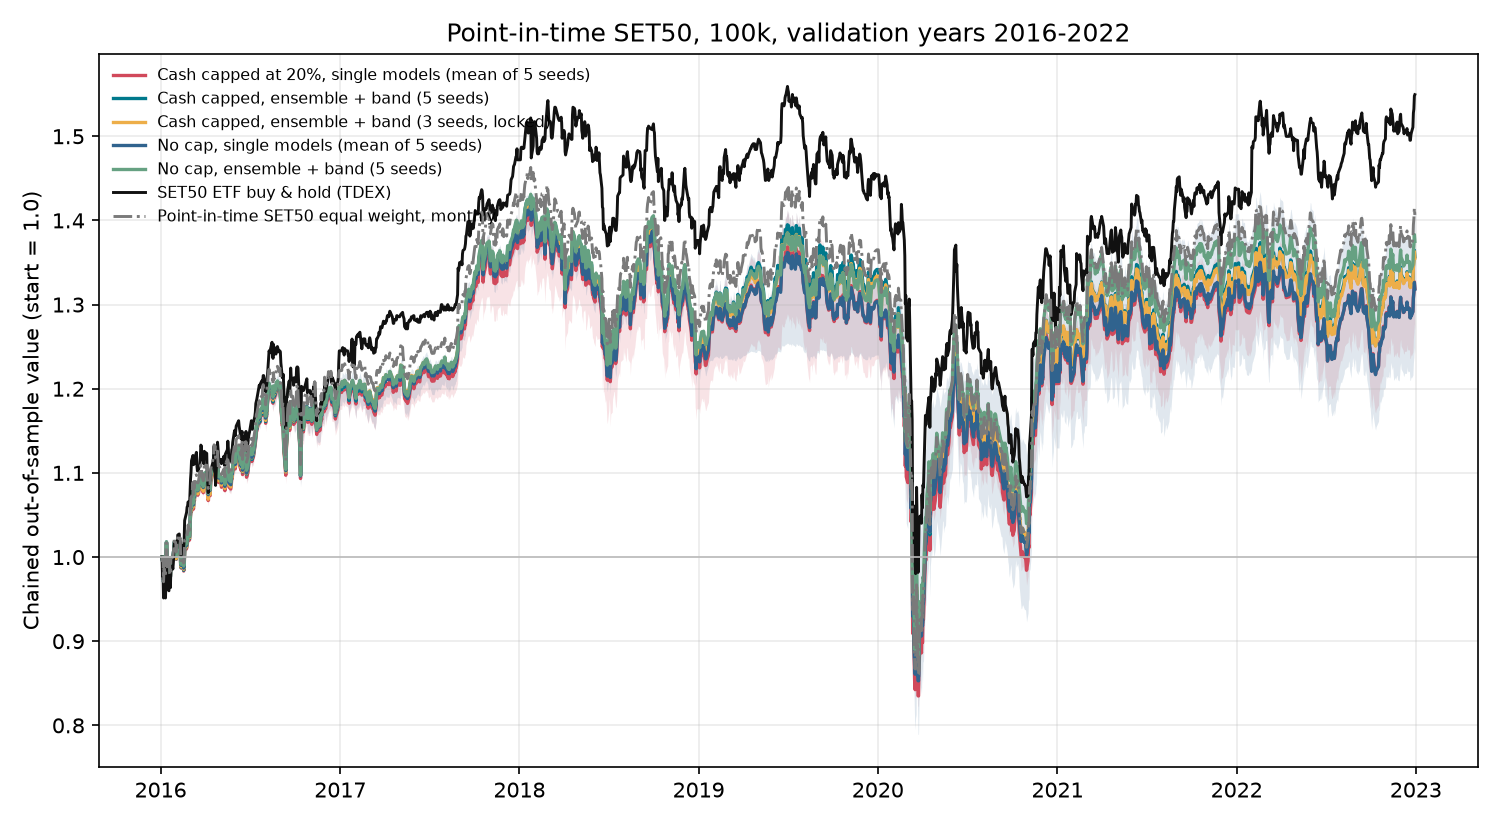
\includegraphics[width=\textwidth]{docs/figures/pit_cash_cap_100k_5seeds_chained_equity_20261126.png}
\end{center}
\footnotesize The cash-capped design (five seeds: single models and the seed ensemble with the band) and the uncapped design, against equal weight and the ETF; each year uses models trained only on earlier years, net of costs.
\end{frame}

\begin{frame}{What The Agent Learned}
\begin{itemize}
  \item \textbf{Close to equal weight:} daily correlation 0.998, about 44 effective holdings of 44.5 tradable members, no weight above about 3\%.
  \item \textbf{Less trading:} the seed ensemble with the band turned over 0.6 times its capital a year after entry (equal weight 0.9).
  \item \textbf{Cash was a learned bias:} 15 models across four designs held 36--94\% cash; shuffling their inputs moved that cash by 5 points or less in 12 of them.
  \item \textbf{The 20\% cash cap} removed the cash-heavy models but not the gap to equal weight, which lies in costs and stock tilts that do not pay.
\end{itemize}
\end{frame}

\begin{frame}{Five Algorithms On BistKA (300k Timesteps, 5 Seeds)}
\begin{center}
\scriptsize
\begin{tabular}{lrrrrr}
\toprule
Five stocks, 2016--2022 & A2C & PPO & SAC & TD3 & DDPG \\
\midrule
Annual return & \textbf{8.7\%} & 4.4\% & 0.3\% & $-0.9\%$ & $-1.4\%$ \\
Costs a year (points) & 0.9 & 1.3 & 6.1 & 6.6 & 6.3 \\
Turnover a year & 4.3 & 6.0 & 29.4 & 32.1 & 30.5 \\
Hours per model & 0.4 & 1.1 & 17.2 & 10.7 & 13.9 \\
\bottomrule
\end{tabular}
\end{center}
\begin{itemize}
  \item ETF 7.1\%, equal weight 10.1\%.
  \item Off-policy algorithms overtraded; TD3 and DDPG are significantly worse than the ETF, equal weight and PPO.
  \item A2C is best and cheapest, but not significantly better than PPO or either benchmark.
\end{itemize}
\end{frame}

\begin{frame}{Longer Training Did Not Help}
\begin{itemize}
  \item \textbf{PPO, five stocks:} 7.6\% a year at 100k timesteps, 4.4\% at 300k; average cash rose from 20\% to 39\%. The only significant budget effect ($-0.16$ Sharpe).
  \item \textbf{Point-in-time, no cap:} at 300k, 17 of 35 models held 45--98\% cash; the ensemble made 3.9\% a year with a smaller drawdown.
  \item \textbf{Point-in-time, 20\% cap:} cash held to 8.7\%, but the ensemble made 4.9\% against 5.0\% at 100k (Sharpe 0.35 against 0.36).
  \item 100k timesteps is enough for the locked design.
\end{itemize}
\end{frame}

\begin{frame}{Choosing The Design Before Looking}
\begin{itemize}
  \item \textbf{Rule fixed in advance (decision 7):} median over years of the annual excess log return over equal weight; if no design scores above zero, equal weight is selected.
  \item \textbf{Outcome:} no DRL design scored above zero in either universe, so the rule selects equal weight.
  \item \textbf{Evaluated anyway:} the best DRL designs, the cash-capped point-in-time ensemble with the band and five-stock A2C at 300k.
  \item \textbf{Locks and gates:} each evaluation ran once from an approved lock file; every opening is in \texttt{results/FINAL\_TEST\_LEDGER.jsonl}.
\end{itemize}
\end{frame}

\begin{frame}{Test Years 2023--2024 (Run Once)}
\begin{center}
\scriptsize
\begin{tabular}{lrrrr}
\toprule
Strategy & 2023 & 2024 & Two years & Sharpe \\
\midrule
\multicolumn{5}{l}{\emph{Point-in-time SET50}} \\
DRL, cash-capped, ensemble + band & $-11.4\%$ & $-6.7\%$ & 0.827 & $-0.80$ \\
Equal weight, monthly & $-13.5\%$ & $-7.6\%$ & 0.799 & $-0.86$ \\
\multicolumn{5}{l}{\emph{Five starter stocks}} \\
DRL, A2C, 300k & $-1.9\%$ & $+4.4\%$ & 1.026 & 0.19 \\
Equal weight, monthly & $-3.6\%$ & $+10.1\%$ & 1.061 & 0.33 \\
\midrule
SET50 ETF buy-and-hold & $-9.1\%$ & $+8.2\%$ & 0.984 & $-0.01$ \\
\bottomrule
\end{tabular}
\end{center}
\begin{itemize}
  \item Point-in-time DRL was ahead of equal weight in both years, not significantly, and behind the ETF.
  \item Yahoo's 2024 prices have stale rows on real trading days; disclosed, results stand as locked.
\end{itemize}
\end{frame}

\begin{frame}{Sealed Holdout, 2025 To 4 November 2026 (Run Once)}
\begin{center}
\scriptsize
\begin{tabular}{lrrrr}
\toprule
Strategy & 2025 & 2026 to 4 Nov & Chained & Sharpe \\
\midrule
\multicolumn{5}{l}{\emph{Point-in-time SET50 (2024 H2 list held fixed)}} \\
DRL, cash-capped, ensemble + band & $-8.8\%$ & $+23.7\%$ & 1.128 & 0.48 \\
Equal weight, monthly & $-8.8\%$ & $+29.7\%$ & 1.183 & 0.60 \\
\multicolumn{5}{l}{\emph{Five starter stocks}} \\
DRL, A2C, 300k & $+0.7\%$ & $+14.3\%$ & 1.153 & 0.59 \\
Equal weight, monthly & $+6.0\%$ & $+20.8\%$ & 1.281 & 0.94 \\
\midrule
SET50 ETF buy-and-hold & $-2.8\%$ & $+24.9\%$ & 1.214 & 0.75 \\
\bottomrule
\end{tabular}
\end{center}
\begin{itemize}
  \item The locked design matched equal weight in the falling year and trailed it in the rally, holding cash up to its cap.
  \item Its Sharpe shortfall against equal weight is \textbf{significant}: $-0.12$ ($-0.23$ to $-0.01$).
\end{itemize}
\end{frame}

\begin{frame}{Sealed Holdout: Chained Value}
\begin{center}
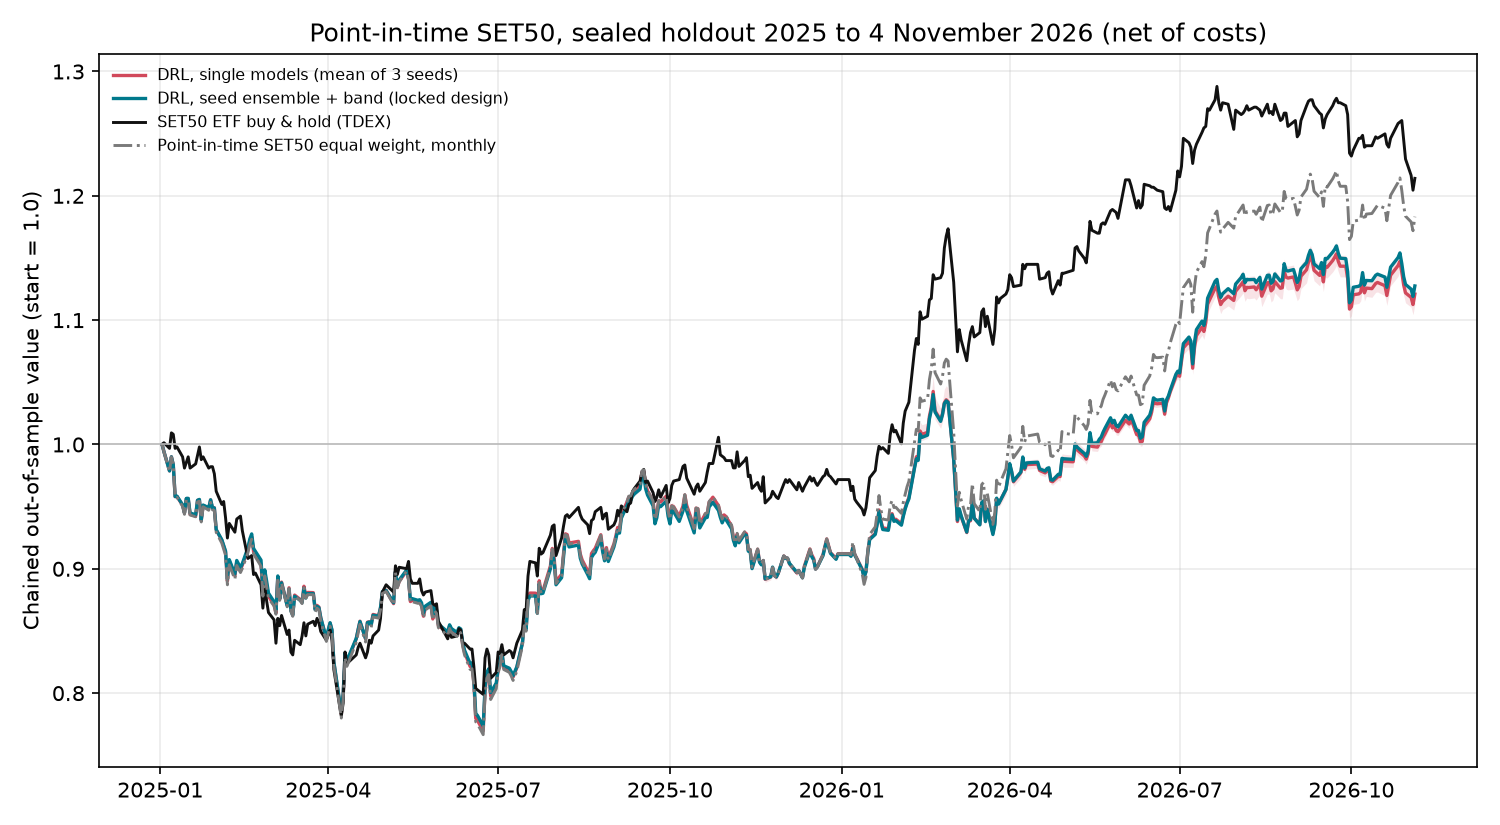
\includegraphics[width=\textwidth]{docs/figures/holdout_pit_chained_equity_20261126.png}
\end{center}
\footnotesize Locked point-in-time design (seed ensemble with the band, and its single models) against equal weight and the ETF; models trained only on earlier years, net of costs.
\end{frame}

\begin{frame}{Checks After The Holdout (Validation Years Only)}
\begin{center}
\scriptsize
\begin{tabular}{lrrr}
\toprule
Locked design with one change (5 seeds) & Single & Ensemble & Sharpe diff. (single) \\
\midrule
Locked: LSTM, technical + ETF inputs & 4.6\% & 5.0\% & -- \\
MLP encoder instead of LSTM & 4.4\% & 5.1\% & $-0.006$ \\
Technical inputs only & 4.5\% & 5.2\% & $-0.001$ \\
+ BOT policy rate & 4.6\% & 5.2\% & $+0.007$ \\
+ daily macro proxies & 4.4\% & 5.0\% & $-0.012$ \\
+ policy rate + macro proxies & 4.6\% & 5.5\% & $+0.018$ \\
+ sector inputs (dated SET sectors) & 4.5\% & 5.1\% & $-0.005$ \\
\midrule
Equal weight, monthly & \multicolumn{2}{r}{5.6\%} & \\
\bottomrule
\end{tabular}
\end{center}
\begin{itemize}
  \item No change is significant. Within the BistKA run, no data source helped over technical inputs alone.
  \item The all-sources ensemble's lead (Sharpe 0.41 against 0.38 for equal weight) came from cash; not significant against the technical-only ensemble.
  \item The models read the sector inputs (shuffling them moved the portfolio by 2.4\%) but gained nothing from them.
\end{itemize}
\end{frame}

\begin{frame}{BistKA Compute And Reproducibility}
\begin{itemize}
  \item \textbf{Job 4409:} 210 models, 1{,}776 task-hours in 56 hours on 32 CPUs, about 2{,}465 service hours.
  \item \textbf{Job 4518:} 35 cash-capped models at 300k, 11.2 hours, 450 service hours.
  \item \textbf{Job 4528:} 147 models (source ablation and a retrain), 14.0 hours, 561 service hours.
  \item \textbf{Across machines:} BistKA's models replay on the Mac to within $10^{-8}$. Retraining the locked design there gave 4.8\% a year against 5.0\% on the Mac: the same result, not the same files.
  \item \textbf{Same machine:} a retrained model was byte-identical.
\end{itemize}
\end{frame}

\begin{frame}{Answers To The Research Questions}
\begin{center}
\scriptsize
\begin{tabular}{p{0.06\textwidth}p{0.82\textwidth}}
\toprule
RQ & Short answer \\
\midrule
1 & Profitable in absolute terms, but no better than equal weight or the SET50 ETF on unseen years. \\
2 & No measurable gain from extra sources; market context helped only on five stocks, borderline. \\
3 & Technical inputs carry the agent; no tested source added value on the point-in-time index. \\
4 & On-policy (A2C, PPO) over off-policy (SAC, TD3, DDPG), which overtrade. \\
5 & Behaviour stable across regimes, but no regime skill; crash-year gains came from seed-dependent cash. \\
6 & Yes for training: three BistKA jobs, models replay across machines; no tuning or sentiment run there. \\
\bottomrule
\end{tabular}
\end{center}
\end{frame}

\begin{frame}{Limitations Of The Extension}
\begin{itemize}
  \item \textbf{Exploratory data:} Yahoo prices, no trading-status or corporate-action records; stale 2024 rows.
  \item \textbf{Survivorship gap:} 13\% of point-in-time member-sessions have no prices.
  \item \textbf{Costs:} 0.20\% per side; no market impact, spreads, board lots or price limits.
  \item \textbf{Sources:} fundamentals, news sentiment and investor flow have no historical data in the window.
  \item \textbf{Selection:} 35 designs tried on the validation years; the deflated Sharpe ratio corrects only in part.
  \item \textbf{Holdout membership:} the 2024 H2 SET50 list was held fixed for 2025--2026.
\end{itemize}
\end{frame}
 after the pilot's Results section.
% Numbers come from the report chapter docs/report_drafts/results_title_alignment_20261106.tex and the
% dated reports it cites (docs/walk_forward_reward_20261106.md, docs/pit_walk_forward_20261107.md,
% docs/bistka_300k_results_20261125.md, docs/final_test_results_20261125.md,
% docs/holdout_results_20261126.md, docs/source_ablation_20261127.md, docs/architecture_ablation_20261127.md).

\section{Extension: Long-Term, Point-in-Time Results}

\begin{frame}{What Changed After The Pilot}
\begin{itemize}
  \item \textbf{Objective:} a long-term reward (log return, a differential Sharpe term, minus new drawdown) with weekly decisions, instead of the one-day reward.
  \item \textbf{Accounting:} self-financing, 0.20\% cost per side, costs charged once.
  \item \textbf{Data:} 2012--2024 history; the official point-in-time SET50 membership (34 lists, 227 tickers).
  \item \textbf{Evaluation:} seven one-year walk-forward folds (2016--2022), each trained only on earlier years; then the 2023--2024 test years and a sealed holdout (2025 to 4 November 2026), each read once.
  \item \textbf{Compute:} the large runs on BistKA (210, 35 and 147 models in three jobs).
\end{itemize}
\end{frame}

\begin{frame}{Reward And Rebalancing Designs (2020--2022)}
\begin{center}
\scriptsize
\begin{tabular}{lrr}
\toprule
Design (PPO, 3 seeds, five stocks) & Return 2020--2022 & Costs \\
\midrule
V2 objective (one-day reward) & $-48.8\% \pm 7.6$ & 75.3\% \\
Daily simple return, fixed accounting & $-41.9\% \pm 6.9$ & 56.0\% \\
Log return, weekly & $-2.8\% \pm 5.8$ & 16.0\% \\
Plan reward, weekly & $-8.8\% \pm 17.2$ & 11.7\% \\
Plan reward, weekly, per-stock LSTM & $+1.9\% \pm 1.1$ & 1.6\% \\
\midrule
SET50 ETF buy-and-hold & $+9.0\%$ & 0.2\% \\
Equal weight, monthly & $+2.7\%$ & 0.5\% \\
\bottomrule
\end{tabular}
\end{center}
\begin{itemize}
  \item The pilot lost money mainly by overtrading. Weekly long-horizon rewards cut costs by 79--94\%.
\end{itemize}
\end{frame}

\begin{frame}{Seven-Year Walk-Forward, Five Stocks}
\begin{center}
\scriptsize
\begin{tabular}{lrrr}
\toprule
Strategy (2016--2022, 7 folds) & Annual return & Years ahead of ETF & Max DD \\
\midrule
LSTM forecast, top two & 13.8\% & 5/7 & $-17.0\%$ \\
Ridge forecast, top two & 12.8\% & 5/7 & $-16.8\%$ \\
Equal weight, monthly & 10.1\% & 4/7 & $-13.9\%$ \\
DRL, plan reward + LSTM (5 seeds) & 7.6\% & 3/7 & $-11.1\%$ \\
SET50 ETF buy-and-hold & 7.1\% & -- & $-11.3\%$ \\
\bottomrule
\end{tabular}
\end{center}
\begin{itemize}
  \item DRL had the lowest drawdown but did not beat equal weight or the forecasters.
  \item No difference is statistically significant (block bootstrap on daily returns).
\end{itemize}
\end{frame}

\begin{frame}{Why The Universe Matters}
\begin{itemize}
  \item Five stocks, or today's SET50 names, are chosen with hindsight.
  \item Equal weight over the \textbf{2024 SET50 names}: 12.2\% a year, ahead of the ETF in 7 of 7 years.
  \item Equal weight over \textbf{each session's actual members}: 5.6\% a year, ahead in 2 of 7.
  \item Hindsight therefore added 6.6 points a year. Every later result uses the actual members.
  \item Gap: 38 of the 227 tickers, mostly delisted or merged, have no Yahoo prices (13\% of member-sessions).
\end{itemize}
\end{frame}

\begin{frame}{Point-in-Time SET50: Design Steps}
\begin{center}
\scriptsize
\begin{tabular}{lrr}
\toprule
Design (validation 2016--2022) & Annual return & Max DD \\
\midrule
DRL, slots ordered by traded value & $-1.1\%$ & $-14.8\%$ \\
+ sticky slot order & 3.7\% & $-14.2\%$ \\
+ shared-weight actor (scores every stock alike) & 4.6\% & $-11.7\%$ \\
+ seed ensemble and 0.5-point no-trade band & 5.5\% & $-11.3\%$ \\
\textbf{+ cash capped at 20\% (locked design)} & \textbf{5.0\%} & $-12.0\%$ \\
Shared actor at 300k timesteps, ensemble + band & 3.9\% & $-7.0\%$ \\
\midrule
Equal weight (point-in-time), monthly & 5.6\% & $-12.7\%$ \\
SET50 ETF buy-and-hold & 7.1\% & $-11.2\%$ \\
Momentum / inverse volatility / minimum variance & 5.3 / 5.0 / 4.0\% & \\
\bottomrule
\end{tabular}
\end{center}
\begin{itemize}
  \item No design beat equal weight; none of these differences is significant except the first two (worse).
\end{itemize}
\end{frame}

\begin{frame}{Point-in-Time SET50: Chained Value}
\begin{center}
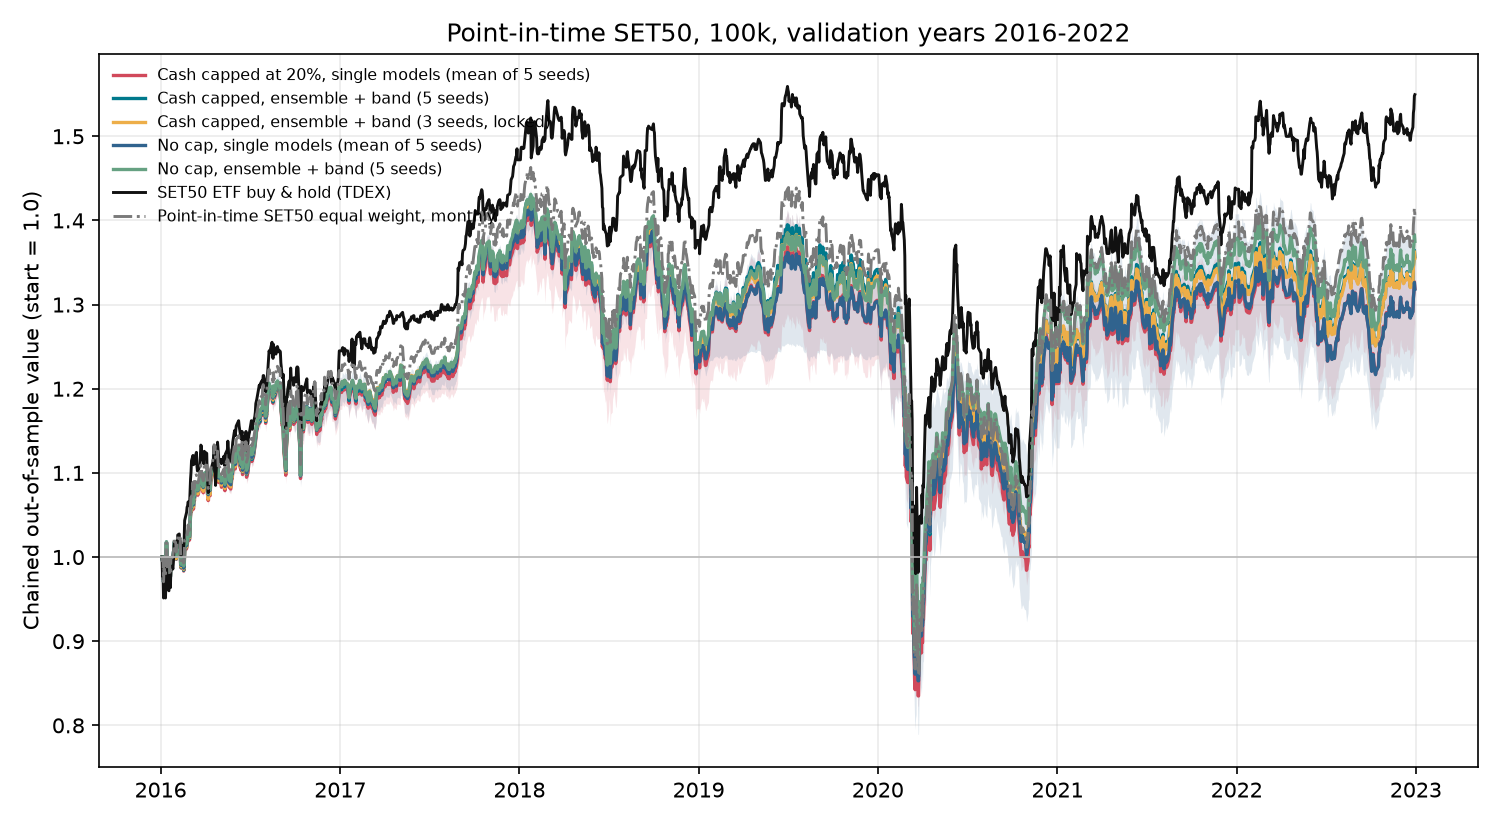
\includegraphics[width=\textwidth]{docs/figures/pit_cash_cap_100k_5seeds_chained_equity_20261126.png}
\end{center}
\footnotesize The cash-capped design (five seeds: single models and the seed ensemble with the band) and the uncapped design, against equal weight and the ETF; each year uses models trained only on earlier years, net of costs.
\end{frame}

\begin{frame}{What The Agent Learned}
\begin{itemize}
  \item \textbf{Close to equal weight:} daily correlation 0.998, about 44 effective holdings of 44.5 tradable members, no weight above about 3\%.
  \item \textbf{Less trading:} the seed ensemble with the band turned over 0.6 times its capital a year after entry (equal weight 0.9).
  \item \textbf{Cash was a learned bias:} 15 models across four designs held 36--94\% cash; shuffling their inputs moved that cash by 5 points or less in 12 of them.
  \item \textbf{The 20\% cash cap} removed the cash-heavy models but not the gap to equal weight, which lies in costs and stock tilts that do not pay.
\end{itemize}
\end{frame}

\begin{frame}{Five Algorithms On BistKA (300k Timesteps, 5 Seeds)}
\begin{center}
\scriptsize
\begin{tabular}{lrrrrr}
\toprule
Five stocks, 2016--2022 & A2C & PPO & SAC & TD3 & DDPG \\
\midrule
Annual return & \textbf{8.7\%} & 4.4\% & 0.3\% & $-0.9\%$ & $-1.4\%$ \\
Costs a year (points) & 0.9 & 1.3 & 6.1 & 6.6 & 6.3 \\
Turnover a year & 4.3 & 6.0 & 29.4 & 32.1 & 30.5 \\
Hours per model & 0.4 & 1.1 & 17.2 & 10.7 & 13.9 \\
\bottomrule
\end{tabular}
\end{center}
\begin{itemize}
  \item ETF 7.1\%, equal weight 10.1\%.
  \item Off-policy algorithms overtraded; TD3 and DDPG are significantly worse than the ETF, equal weight and PPO.
  \item A2C is best and cheapest, but not significantly better than PPO or either benchmark.
\end{itemize}
\end{frame}

\begin{frame}{Longer Training Did Not Help}
\begin{itemize}
  \item \textbf{PPO, five stocks:} 7.6\% a year at 100k timesteps, 4.4\% at 300k; average cash rose from 20\% to 39\%. The only significant budget effect ($-0.16$ Sharpe).
  \item \textbf{Point-in-time, no cap:} at 300k, 17 of 35 models held 45--98\% cash; the ensemble made 3.9\% a year with a smaller drawdown.
  \item \textbf{Point-in-time, 20\% cap:} cash held to 8.7\%, but the ensemble made 4.9\% against 5.0\% at 100k (Sharpe 0.35 against 0.36).
  \item 100k timesteps is enough for the locked design.
\end{itemize}
\end{frame}

\begin{frame}{Choosing The Design Before Looking}
\begin{itemize}
  \item \textbf{Rule fixed in advance (decision 7):} median over years of the annual excess log return over equal weight; if no design scores above zero, equal weight is selected.
  \item \textbf{Outcome:} no DRL design scored above zero in either universe, so the rule selects equal weight.
  \item \textbf{Evaluated anyway:} the best DRL designs, the cash-capped point-in-time ensemble with the band and five-stock A2C at 300k.
  \item \textbf{Locks and gates:} each evaluation ran once from an approved lock file; every opening is in \texttt{results/FINAL\_TEST\_LEDGER.jsonl}.
\end{itemize}
\end{frame}

\begin{frame}{Test Years 2023--2024 (Run Once)}
\begin{center}
\scriptsize
\begin{tabular}{lrrrr}
\toprule
Strategy & 2023 & 2024 & Two years & Sharpe \\
\midrule
\multicolumn{5}{l}{\emph{Point-in-time SET50}} \\
DRL, cash-capped, ensemble + band & $-11.4\%$ & $-6.7\%$ & 0.827 & $-0.80$ \\
Equal weight, monthly & $-13.5\%$ & $-7.6\%$ & 0.799 & $-0.86$ \\
\multicolumn{5}{l}{\emph{Five starter stocks}} \\
DRL, A2C, 300k & $-1.9\%$ & $+4.4\%$ & 1.026 & 0.19 \\
Equal weight, monthly & $-3.6\%$ & $+10.1\%$ & 1.061 & 0.33 \\
\midrule
SET50 ETF buy-and-hold & $-9.1\%$ & $+8.2\%$ & 0.984 & $-0.01$ \\
\bottomrule
\end{tabular}
\end{center}
\begin{itemize}
  \item Point-in-time DRL was ahead of equal weight in both years, not significantly, and behind the ETF.
  \item Yahoo's 2024 prices have stale rows on real trading days; disclosed, results stand as locked.
\end{itemize}
\end{frame}

\begin{frame}{Sealed Holdout, 2025 To 4 November 2026 (Run Once)}
\begin{center}
\scriptsize
\begin{tabular}{lrrrr}
\toprule
Strategy & 2025 & 2026 to 4 Nov & Chained & Sharpe \\
\midrule
\multicolumn{5}{l}{\emph{Point-in-time SET50 (2024 H2 list held fixed)}} \\
DRL, cash-capped, ensemble + band & $-8.8\%$ & $+23.7\%$ & 1.128 & 0.48 \\
Equal weight, monthly & $-8.8\%$ & $+29.7\%$ & 1.183 & 0.60 \\
\multicolumn{5}{l}{\emph{Five starter stocks}} \\
DRL, A2C, 300k & $+0.7\%$ & $+14.3\%$ & 1.153 & 0.59 \\
Equal weight, monthly & $+6.0\%$ & $+20.8\%$ & 1.281 & 0.94 \\
\midrule
SET50 ETF buy-and-hold & $-2.8\%$ & $+24.9\%$ & 1.214 & 0.75 \\
\bottomrule
\end{tabular}
\end{center}
\begin{itemize}
  \item The locked design matched equal weight in the falling year and trailed it in the rally, holding cash up to its cap.
  \item Its Sharpe shortfall against equal weight is \textbf{significant}: $-0.12$ ($-0.23$ to $-0.01$).
\end{itemize}
\end{frame}

\begin{frame}{Sealed Holdout: Chained Value}
\begin{center}
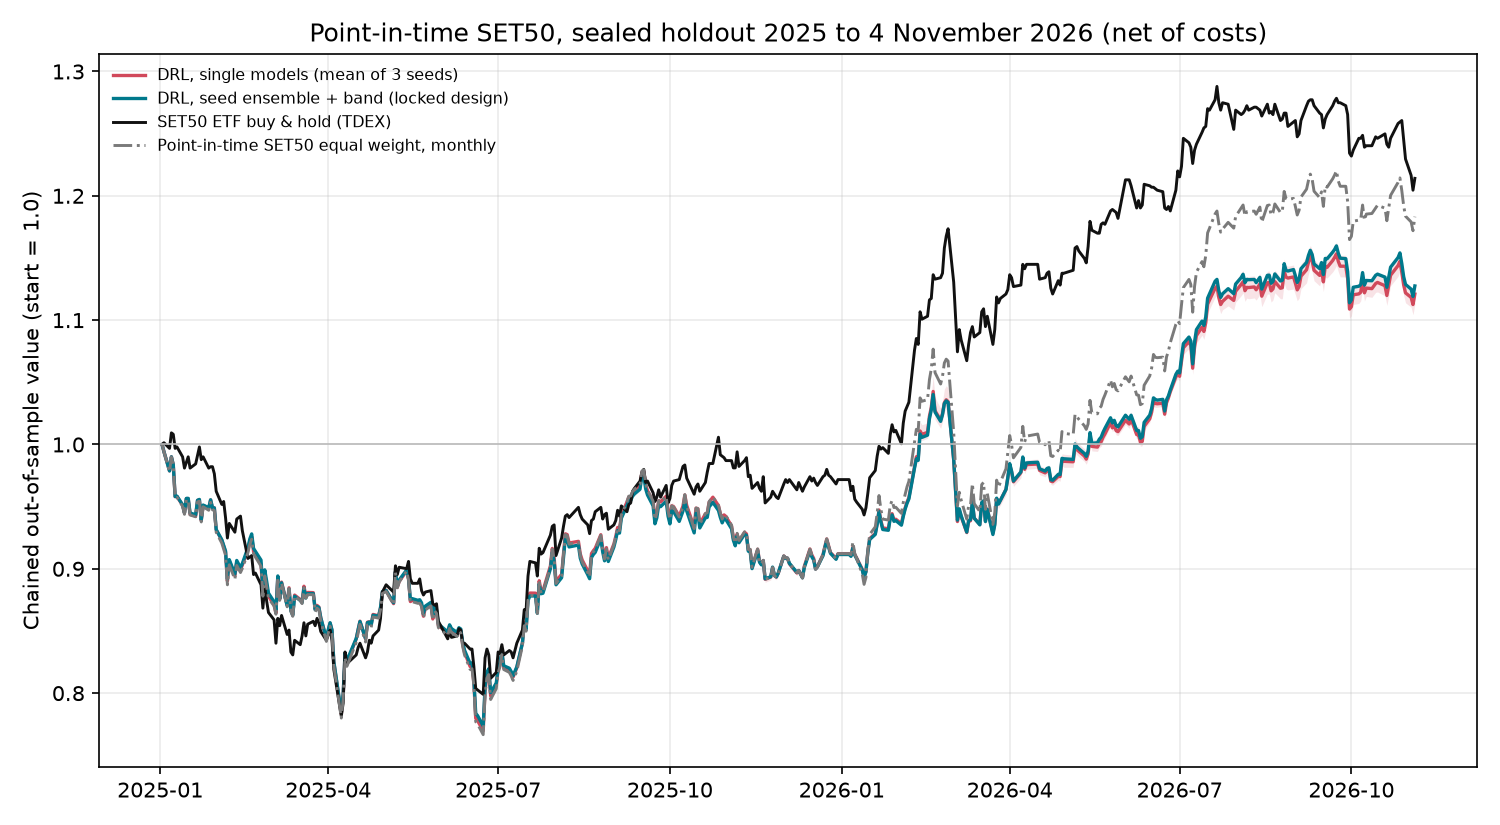
\includegraphics[width=\textwidth]{docs/figures/holdout_pit_chained_equity_20261126.png}
\end{center}
\footnotesize Locked point-in-time design (seed ensemble with the band, and its single models) against equal weight and the ETF; models trained only on earlier years, net of costs.
\end{frame}

\begin{frame}{Checks After The Holdout (Validation Years Only)}
\begin{center}
\scriptsize
\begin{tabular}{lrrr}
\toprule
Locked design with one change (5 seeds) & Single & Ensemble & Sharpe diff. (single) \\
\midrule
Locked: LSTM, technical + ETF inputs & 4.6\% & 5.0\% & -- \\
MLP encoder instead of LSTM & 4.4\% & 5.1\% & $-0.006$ \\
Technical inputs only & 4.5\% & 5.2\% & $-0.001$ \\
+ BOT policy rate & 4.6\% & 5.2\% & $+0.007$ \\
+ daily macro proxies & 4.4\% & 5.0\% & $-0.012$ \\
+ policy rate + macro proxies & 4.6\% & 5.5\% & $+0.018$ \\
+ sector inputs (dated SET sectors) & 4.5\% & 5.1\% & $-0.005$ \\
\midrule
Equal weight, monthly & \multicolumn{2}{r}{5.6\%} & \\
\bottomrule
\end{tabular}
\end{center}
\begin{itemize}
  \item No change is significant. Within the BistKA run, no data source helped over technical inputs alone.
  \item The all-sources ensemble's lead (Sharpe 0.41 against 0.38 for equal weight) came from cash; not significant against the technical-only ensemble.
  \item The models read the sector inputs (shuffling them moved the portfolio by 2.4\%) but gained nothing from them.
\end{itemize}
\end{frame}

\begin{frame}{BistKA Compute And Reproducibility}
\begin{itemize}
  \item \textbf{Job 4409:} 210 models, 1{,}776 task-hours in 56 hours on 32 CPUs, about 2{,}465 service hours.
  \item \textbf{Job 4518:} 35 cash-capped models at 300k, 11.2 hours, 450 service hours.
  \item \textbf{Job 4528:} 147 models (source ablation and a retrain), 14.0 hours, 561 service hours.
  \item \textbf{Across machines:} BistKA's models replay on the Mac to within $10^{-8}$. Retraining the locked design there gave 4.8\% a year against 5.0\% on the Mac: the same result, not the same files.
  \item \textbf{Same machine:} a retrained model was byte-identical.
\end{itemize}
\end{frame}

\begin{frame}{Answers To The Research Questions}
\begin{center}
\scriptsize
\begin{tabular}{p{0.06\textwidth}p{0.82\textwidth}}
\toprule
RQ & Short answer \\
\midrule
1 & Profitable in absolute terms, but no better than equal weight or the SET50 ETF on unseen years. \\
2 & No measurable gain from extra sources; market context helped only on five stocks, borderline. \\
3 & Technical inputs carry the agent; no tested source added value on the point-in-time index. \\
4 & On-policy (A2C, PPO) over off-policy (SAC, TD3, DDPG), which overtrade. \\
5 & Behaviour stable across regimes, but no regime skill; crash-year gains came from seed-dependent cash. \\
6 & Yes for training: three BistKA jobs, models replay across machines; no tuning or sentiment run there. \\
\bottomrule
\end{tabular}
\end{center}
\end{frame}

\begin{frame}{Limitations Of The Extension}
\begin{itemize}
  \item \textbf{Exploratory data:} Yahoo prices, no trading-status or corporate-action records; stale 2024 rows.
  \item \textbf{Survivorship gap:} 13\% of point-in-time member-sessions have no prices.
  \item \textbf{Costs:} 0.20\% per side; no market impact, spreads, board lots or price limits.
  \item \textbf{Sources:} fundamentals, news sentiment and investor flow have no historical data in the window.
  \item \textbf{Selection:} 35 designs tried on the validation years; the deflated Sharpe ratio corrects only in part.
  \item \textbf{Holdout membership:} the 2024 H2 SET50 list was held fixed for 2025--2026.
\end{itemize}
\end{frame}
 after the pilot's Results section.
% Numbers come from the report chapter docs/report_drafts/results_title_alignment_20261106.tex and the
% dated reports it cites (docs/walk_forward_reward_20261106.md, docs/pit_walk_forward_20261107.md,
% docs/bistka_300k_results_20261125.md, docs/final_test_results_20261125.md,
% docs/holdout_results_20261126.md, docs/source_ablation_20261127.md, docs/architecture_ablation_20261127.md).

\section{Extension: Long-Term, Point-in-Time Results}

\begin{frame}{What Changed After The Pilot}
\begin{itemize}
  \item \textbf{Objective:} a long-term reward (log return, a differential Sharpe term, minus new drawdown) with weekly decisions, instead of the one-day reward.
  \item \textbf{Accounting:} self-financing, 0.20\% cost per side, costs charged once.
  \item \textbf{Data:} 2012--2024 history; the official point-in-time SET50 membership (34 lists, 227 tickers).
  \item \textbf{Evaluation:} seven one-year walk-forward folds (2016--2022), each trained only on earlier years; then the 2023--2024 test years and a sealed holdout (2025 to 4 November 2026), each read once.
  \item \textbf{Compute:} the large runs on BistKA (210, 35 and 147 models in three jobs).
\end{itemize}
\end{frame}

\begin{frame}{Reward And Rebalancing Designs (2020--2022)}
\begin{center}
\scriptsize
\begin{tabular}{lrr}
\toprule
Design (PPO, 3 seeds, five stocks) & Return 2020--2022 & Costs \\
\midrule
V2 objective (one-day reward) & $-48.8\% \pm 7.6$ & 75.3\% \\
Daily simple return, fixed accounting & $-41.9\% \pm 6.9$ & 56.0\% \\
Log return, weekly & $-2.8\% \pm 5.8$ & 16.0\% \\
Plan reward, weekly & $-8.8\% \pm 17.2$ & 11.7\% \\
Plan reward, weekly, per-stock LSTM & $+1.9\% \pm 1.1$ & 1.6\% \\
\midrule
SET50 ETF buy-and-hold & $+9.0\%$ & 0.2\% \\
Equal weight, monthly & $+2.7\%$ & 0.5\% \\
\bottomrule
\end{tabular}
\end{center}
\begin{itemize}
  \item The pilot lost money mainly by overtrading. Weekly long-horizon rewards cut costs by 79--94\%.
\end{itemize}
\end{frame}

\begin{frame}{Seven-Year Walk-Forward, Five Stocks}
\begin{center}
\scriptsize
\begin{tabular}{lrrr}
\toprule
Strategy (2016--2022, 7 folds) & Annual return & Years ahead of ETF & Max DD \\
\midrule
LSTM forecast, top two & 13.8\% & 5/7 & $-17.0\%$ \\
Ridge forecast, top two & 12.8\% & 5/7 & $-16.8\%$ \\
Equal weight, monthly & 10.1\% & 4/7 & $-13.9\%$ \\
DRL, plan reward + LSTM (5 seeds) & 7.6\% & 3/7 & $-11.1\%$ \\
SET50 ETF buy-and-hold & 7.1\% & -- & $-11.3\%$ \\
\bottomrule
\end{tabular}
\end{center}
\begin{itemize}
  \item DRL had the lowest drawdown but did not beat equal weight or the forecasters.
  \item No difference is statistically significant (block bootstrap on daily returns).
\end{itemize}
\end{frame}

\begin{frame}{Why The Universe Matters}
\begin{itemize}
  \item Five stocks, or today's SET50 names, are chosen with hindsight.
  \item Equal weight over the \textbf{2024 SET50 names}: 12.2\% a year, ahead of the ETF in 7 of 7 years.
  \item Equal weight over \textbf{each session's actual members}: 5.6\% a year, ahead in 2 of 7.
  \item Hindsight therefore added 6.6 points a year. Every later result uses the actual members.
  \item Gap: 38 of the 227 tickers, mostly delisted or merged, have no Yahoo prices (13\% of member-sessions).
\end{itemize}
\end{frame}

\begin{frame}{Point-in-Time SET50: Design Steps}
\begin{center}
\scriptsize
\begin{tabular}{lrr}
\toprule
Design (validation 2016--2022) & Annual return & Max DD \\
\midrule
DRL, slots ordered by traded value & $-1.1\%$ & $-14.8\%$ \\
+ sticky slot order & 3.7\% & $-14.2\%$ \\
+ shared-weight actor (scores every stock alike) & 4.6\% & $-11.7\%$ \\
+ seed ensemble and 0.5-point no-trade band & 5.5\% & $-11.3\%$ \\
\textbf{+ cash capped at 20\% (locked design)} & \textbf{5.0\%} & $-12.0\%$ \\
Shared actor at 300k timesteps, ensemble + band & 3.9\% & $-7.0\%$ \\
\midrule
Equal weight (point-in-time), monthly & 5.6\% & $-12.7\%$ \\
SET50 ETF buy-and-hold & 7.1\% & $-11.2\%$ \\
Momentum / inverse volatility / minimum variance & 5.3 / 5.0 / 4.0\% & \\
\bottomrule
\end{tabular}
\end{center}
\begin{itemize}
  \item No design beat equal weight; none of these differences is significant except the first two (worse).
\end{itemize}
\end{frame}

\begin{frame}{Point-in-Time SET50: Chained Value}
\begin{center}
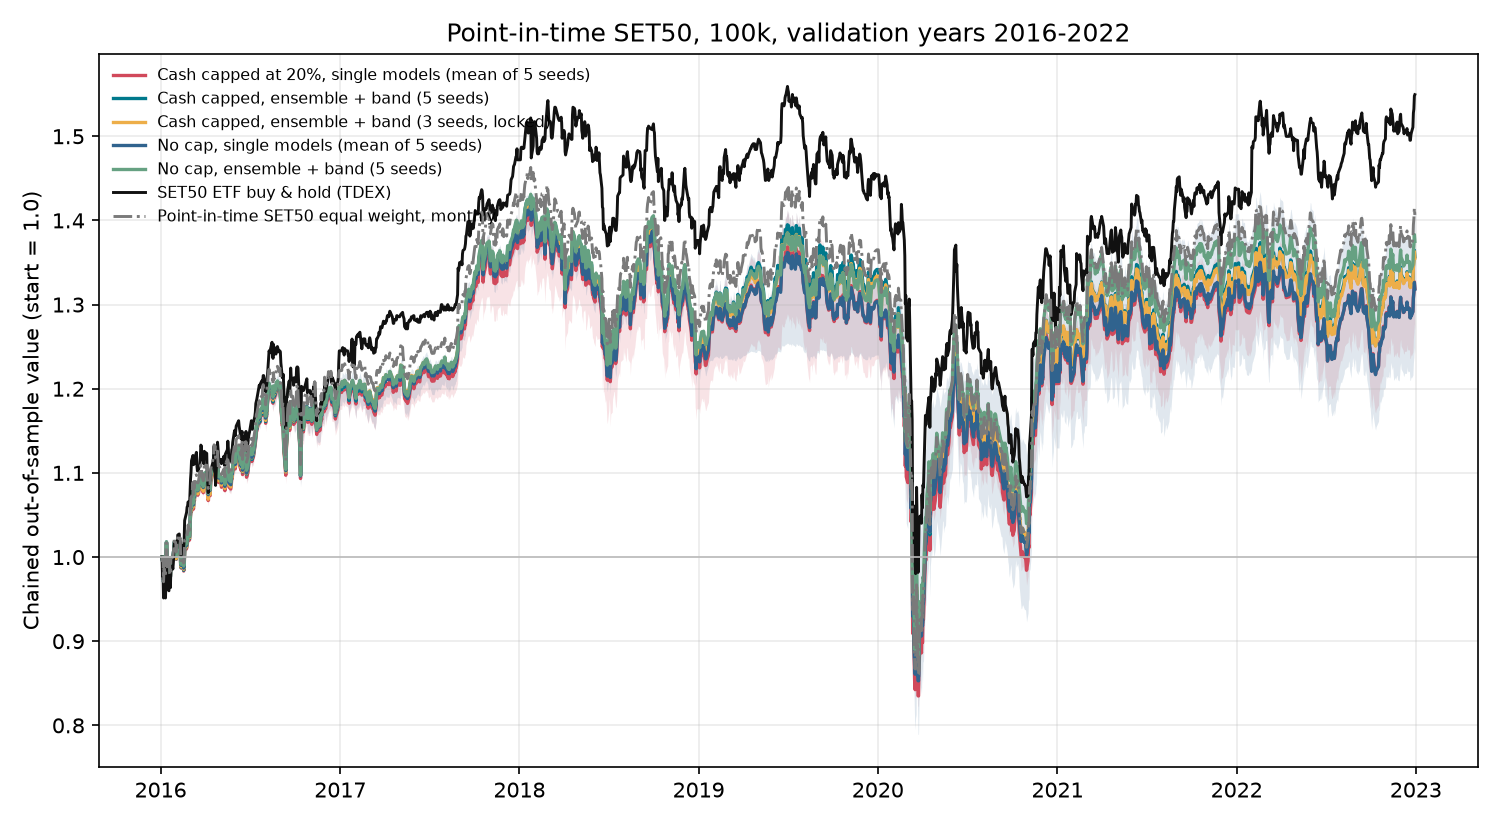
\includegraphics[width=\textwidth]{docs/figures/pit_cash_cap_100k_5seeds_chained_equity_20261126.png}
\end{center}
\footnotesize The cash-capped design (five seeds: single models and the seed ensemble with the band) and the uncapped design, against equal weight and the ETF; each year uses models trained only on earlier years, net of costs.
\end{frame}

\begin{frame}{What The Agent Learned}
\begin{itemize}
  \item \textbf{Close to equal weight:} daily correlation 0.998, about 44 effective holdings of 44.5 tradable members, no weight above about 3\%.
  \item \textbf{Less trading:} the seed ensemble with the band turned over 0.6 times its capital a year after entry (equal weight 0.9).
  \item \textbf{Cash was a learned bias:} 15 models across four designs held 36--94\% cash; shuffling their inputs moved that cash by 5 points or less in 12 of them.
  \item \textbf{The 20\% cash cap} removed the cash-heavy models but not the gap to equal weight, which lies in costs and stock tilts that do not pay.
\end{itemize}
\end{frame}

\begin{frame}{Five Algorithms On BistKA (300k Timesteps, 5 Seeds)}
\begin{center}
\scriptsize
\begin{tabular}{lrrrrr}
\toprule
Five stocks, 2016--2022 & A2C & PPO & SAC & TD3 & DDPG \\
\midrule
Annual return & \textbf{8.7\%} & 4.4\% & 0.3\% & $-0.9\%$ & $-1.4\%$ \\
Costs a year (points) & 0.9 & 1.3 & 6.1 & 6.6 & 6.3 \\
Turnover a year & 4.3 & 6.0 & 29.4 & 32.1 & 30.5 \\
Hours per model & 0.4 & 1.1 & 17.2 & 10.7 & 13.9 \\
\bottomrule
\end{tabular}
\end{center}
\begin{itemize}
  \item ETF 7.1\%, equal weight 10.1\%.
  \item Off-policy algorithms overtraded; TD3 and DDPG are significantly worse than the ETF, equal weight and PPO.
  \item A2C is best and cheapest, but not significantly better than PPO or either benchmark.
\end{itemize}
\end{frame}

\begin{frame}{Longer Training Did Not Help}
\begin{itemize}
  \item \textbf{PPO, five stocks:} 7.6\% a year at 100k timesteps, 4.4\% at 300k; average cash rose from 20\% to 39\%. The only significant budget effect ($-0.16$ Sharpe).
  \item \textbf{Point-in-time, no cap:} at 300k, 17 of 35 models held 45--98\% cash; the ensemble made 3.9\% a year with a smaller drawdown.
  \item \textbf{Point-in-time, 20\% cap:} cash held to 8.7\%, but the ensemble made 4.9\% against 5.0\% at 100k (Sharpe 0.35 against 0.36).
  \item 100k timesteps is enough for the locked design.
\end{itemize}
\end{frame}

\begin{frame}{Choosing The Design Before Looking}
\begin{itemize}
  \item \textbf{Rule fixed in advance (decision 7):} median over years of the annual excess log return over equal weight; if no design scores above zero, equal weight is selected.
  \item \textbf{Outcome:} no DRL design scored above zero in either universe, so the rule selects equal weight.
  \item \textbf{Evaluated anyway:} the best DRL designs, the cash-capped point-in-time ensemble with the band and five-stock A2C at 300k.
  \item \textbf{Locks and gates:} each evaluation ran once from an approved lock file; every opening is in \texttt{results/FINAL\_TEST\_LEDGER.jsonl}.
\end{itemize}
\end{frame}

\begin{frame}{Test Years 2023--2024 (Run Once)}
\begin{center}
\scriptsize
\begin{tabular}{lrrrr}
\toprule
Strategy & 2023 & 2024 & Two years & Sharpe \\
\midrule
\multicolumn{5}{l}{\emph{Point-in-time SET50}} \\
DRL, cash-capped, ensemble + band & $-11.4\%$ & $-6.7\%$ & 0.827 & $-0.80$ \\
Equal weight, monthly & $-13.5\%$ & $-7.6\%$ & 0.799 & $-0.86$ \\
\multicolumn{5}{l}{\emph{Five starter stocks}} \\
DRL, A2C, 300k & $-1.9\%$ & $+4.4\%$ & 1.026 & 0.19 \\
Equal weight, monthly & $-3.6\%$ & $+10.1\%$ & 1.061 & 0.33 \\
\midrule
SET50 ETF buy-and-hold & $-9.1\%$ & $+8.2\%$ & 0.984 & $-0.01$ \\
\bottomrule
\end{tabular}
\end{center}
\begin{itemize}
  \item Point-in-time DRL was ahead of equal weight in both years, not significantly, and behind the ETF.
  \item Yahoo's 2024 prices have stale rows on real trading days; disclosed, results stand as locked.
\end{itemize}
\end{frame}

\begin{frame}{Sealed Holdout, 2025 To 4 November 2026 (Run Once)}
\begin{center}
\scriptsize
\begin{tabular}{lrrrr}
\toprule
Strategy & 2025 & 2026 to 4 Nov & Chained & Sharpe \\
\midrule
\multicolumn{5}{l}{\emph{Point-in-time SET50 (2024 H2 list held fixed)}} \\
DRL, cash-capped, ensemble + band & $-8.8\%$ & $+23.7\%$ & 1.128 & 0.48 \\
Equal weight, monthly & $-8.8\%$ & $+29.7\%$ & 1.183 & 0.60 \\
\multicolumn{5}{l}{\emph{Five starter stocks}} \\
DRL, A2C, 300k & $+0.7\%$ & $+14.3\%$ & 1.153 & 0.59 \\
Equal weight, monthly & $+6.0\%$ & $+20.8\%$ & 1.281 & 0.94 \\
\midrule
SET50 ETF buy-and-hold & $-2.8\%$ & $+24.9\%$ & 1.214 & 0.75 \\
\bottomrule
\end{tabular}
\end{center}
\begin{itemize}
  \item The locked design matched equal weight in the falling year and trailed it in the rally, holding cash up to its cap.
  \item Its Sharpe shortfall against equal weight is \textbf{significant}: $-0.12$ ($-0.23$ to $-0.01$).
\end{itemize}
\end{frame}

\begin{frame}{Sealed Holdout: Chained Value}
\begin{center}
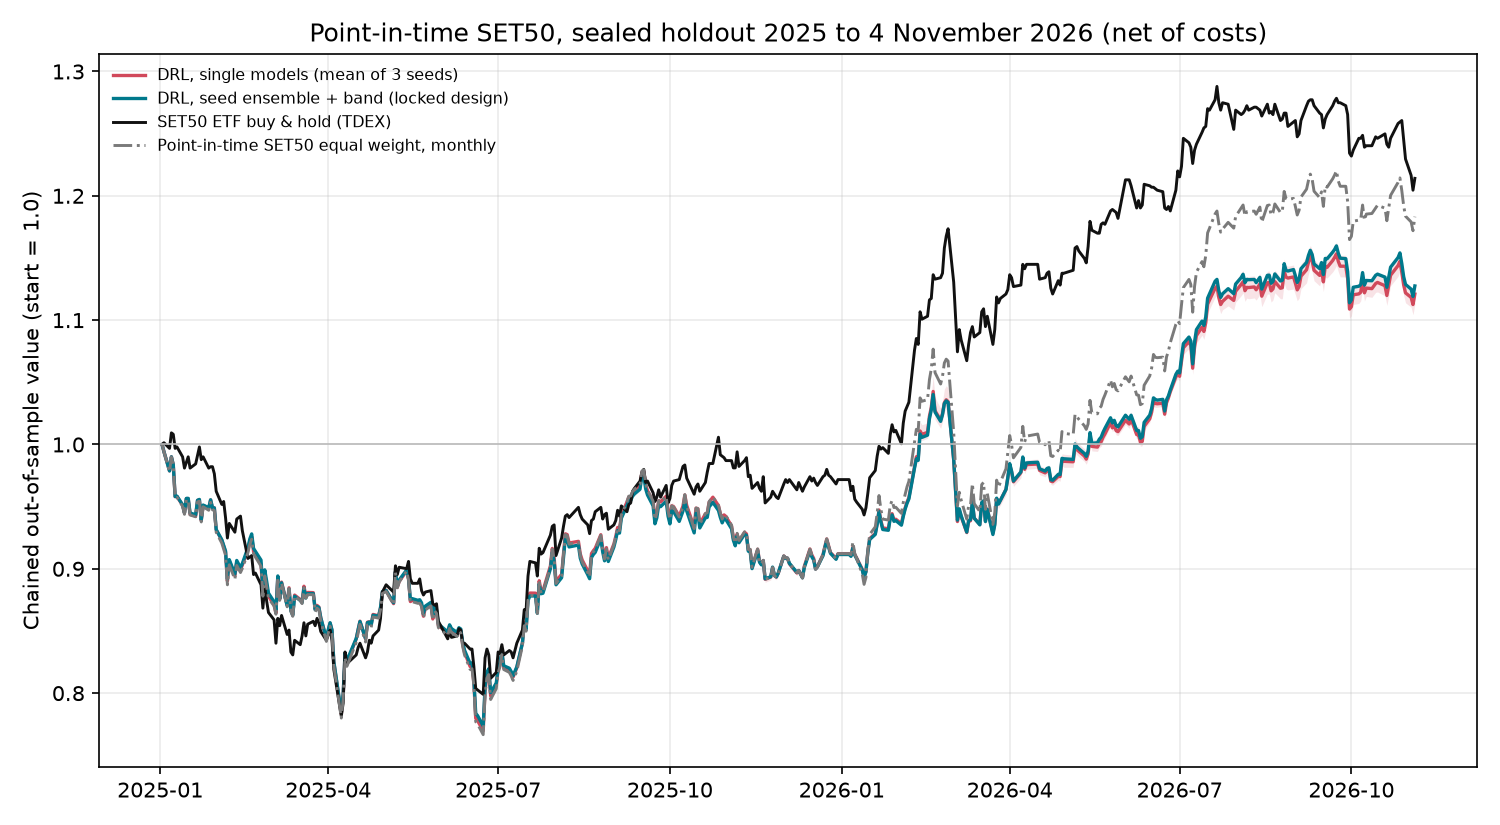
\includegraphics[width=\textwidth]{docs/figures/holdout_pit_chained_equity_20261126.png}
\end{center}
\footnotesize Locked point-in-time design (seed ensemble with the band, and its single models) against equal weight and the ETF; models trained only on earlier years, net of costs.
\end{frame}

\begin{frame}{Checks After The Holdout (Validation Years Only)}
\begin{center}
\scriptsize
\begin{tabular}{lrrr}
\toprule
Locked design with one change (5 seeds) & Single & Ensemble & Sharpe diff. (single) \\
\midrule
Locked: LSTM, technical + ETF inputs & 4.6\% & 5.0\% & -- \\
MLP encoder instead of LSTM & 4.4\% & 5.1\% & $-0.006$ \\
Technical inputs only & 4.5\% & 5.2\% & $-0.001$ \\
+ BOT policy rate & 4.6\% & 5.2\% & $+0.007$ \\
+ daily macro proxies & 4.4\% & 5.0\% & $-0.012$ \\
+ policy rate + macro proxies & 4.6\% & 5.5\% & $+0.018$ \\
+ sector inputs (dated SET sectors) & 4.5\% & 5.1\% & $-0.005$ \\
\midrule
Equal weight, monthly & \multicolumn{2}{r}{5.6\%} & \\
\bottomrule
\end{tabular}
\end{center}
\begin{itemize}
  \item No change is significant. Within the BistKA run, no data source helped over technical inputs alone.
  \item The all-sources ensemble's lead (Sharpe 0.41 against 0.38 for equal weight) came from cash; not significant against the technical-only ensemble.
  \item The models read the sector inputs (shuffling them moved the portfolio by 2.4\%) but gained nothing from them.
\end{itemize}
\end{frame}

\begin{frame}{BistKA Compute And Reproducibility}
\begin{itemize}
  \item \textbf{Job 4409:} 210 models, 1{,}776 task-hours in 56 hours on 32 CPUs, about 2{,}465 service hours.
  \item \textbf{Job 4518:} 35 cash-capped models at 300k, 11.2 hours, 450 service hours.
  \item \textbf{Job 4528:} 147 models (source ablation and a retrain), 14.0 hours, 561 service hours.
  \item \textbf{Across machines:} BistKA's models replay on the Mac to within $10^{-8}$. Retraining the locked design there gave 4.8\% a year against 5.0\% on the Mac: the same result, not the same files.
  \item \textbf{Same machine:} a retrained model was byte-identical.
\end{itemize}
\end{frame}

\begin{frame}{Answers To The Research Questions}
\begin{center}
\scriptsize
\begin{tabular}{p{0.06\textwidth}p{0.82\textwidth}}
\toprule
RQ & Short answer \\
\midrule
1 & Profitable in absolute terms, but no better than equal weight or the SET50 ETF on unseen years. \\
2 & No measurable gain from extra sources; market context helped only on five stocks, borderline. \\
3 & Technical inputs carry the agent; no tested source added value on the point-in-time index. \\
4 & On-policy (A2C, PPO) over off-policy (SAC, TD3, DDPG), which overtrade. \\
5 & Behaviour stable across regimes, but no regime skill; crash-year gains came from seed-dependent cash. \\
6 & Yes for training: three BistKA jobs, models replay across machines; no tuning or sentiment run there. \\
\bottomrule
\end{tabular}
\end{center}
\end{frame}

\begin{frame}{Limitations Of The Extension}
\begin{itemize}
  \item \textbf{Exploratory data:} Yahoo prices, no trading-status or corporate-action records; stale 2024 rows.
  \item \textbf{Survivorship gap:} 13\% of point-in-time member-sessions have no prices.
  \item \textbf{Costs:} 0.20\% per side; no market impact, spreads, board lots or price limits.
  \item \textbf{Sources:} fundamentals, news sentiment and investor flow have no historical data in the window.
  \item \textbf{Selection:} 35 designs tried on the validation years; the deflated Sharpe ratio corrects only in part.
  \item \textbf{Holdout membership:} the 2024 H2 SET50 list was held fixed for 2025--2026.
\end{itemize}
\end{frame}
